\documentclass[a4paper, 12pt]{report}
%\documentclass[a4paper, 12pt, twocolumn]{report}   using multicol package looks better
\usepackage{tikz, amsmath, amssymb, amsthm, enumitem, amsfonts, listings, upquote, graphicx, float, caption, subcaption, upquote, upgreek, tabularx, titlesec, lipsum, multicol, wrapfig}
\usepackage[document]{ragged2e} %left justifies everything automatically
\newenvironment{Figure}	%to make include pictures inside of multicols easy
  {\par\medskip\noindent\minipage{\linewidth}}
  {\endminipage\par\medskip}
  
\setlength\columnsep{20pt}		%horizontal separation for the columns
  
%set the page borders
\usepackage[
top    = 2cm,
bottom = 2cm,
left   = 1.5cm,
right  = 1.5cm, includefoot]{geometry}

%natural number and integer set symbols, type \N or \Z
\newcommand{\N}{\mathbb{N}}
\newcommand{\Z}{\mathbb{Z}}

%any color you want to use, put here
\definecolor{darkgreen}{rgb}{0,0.4,0}
\definecolor{mylighergray}{rgb}{0.85,0.85,0.85}

%For code snippets
\lstset{ 
  backgroundcolor=\color{mylighergray},   	% choose the background color; you must add 
  basicstyle=\small,        					% the size of the fonts that are used for the code
  breakatwhitespace=false,         			% sets if automatic breaks should only happen at whitespace
  breaklines=true,                 				% sets automatic line breaking
  captionpos=b,                    				% sets the caption-position to bottom
  commentstyle=\color{darkgreen},    		% comment style
  deletekeywords={...},            			% if you want to delete keywords from the given language
  escapeinside={\%*}{*)},         			% if you want to add LaTeX within your code
  extendedchars=true,            				% lets you use non-ASCII characters; for 8-bits encodings only, 
  frame=single,	                   				% adds a frame around the code
  keepspaces=true,                 				% keeps spaces in text, useful for keeping indentation of code 
  keywordstyle=\color{blue},       			% keyword style
  language=Octave,                 			% the language of the code
  morekeywords={*,...},            			% if you want to add more keywords to the set
  numbers=left,                    				% where to put the line-numbers; possible values are (none, left, right)
  numbersep=5pt,                   			% how far the line-numbers are from the code
  numberstyle=\tiny\color{gray}, 			% the style that is used for the line-numbers
  rulecolor=\color{black},         			% if not set, the frame-color may be changed on line-breaks within 
  showspaces=false,                				% show spaces everywhere adding particular underscores; it 
  showstringspaces=false,          			% underline spaces within strings only
  showtabs=false,                 				% show tabs within strings adding particular underscores
  stepnumber=1,                   				% the step between two line-numbers. If it's 1, each line will be numbered
  stringstyle=\color{darkgreen},     			% string literal style
  tabsize=1,	                   					% sets default tabsize to 2 spaces
  title=\lstname                   				% show the filename of files included with \lstinputlisting; also try 
}

\begin{document}

%\onecolumn

\begin{center}
{\huge  \textbf{ECS 171 Group Project}} \\
{\large Benjamen Neduva, Calvin Cramer, Lionel Quiambao, Lisa M. Slaughter, \\Maksim Nedorezov, Ryan Gosiaco, Shifan Li, Victoria Salova} \\
Prof. Ilias Tagkopoulos\\
Date quarter year?\\

\end{center}

%General Information
\section{General Information}
\lipsum[1]

%Abstract
\section{Abstract}
\lipsum[2]

%\twocolumn
\begin{multicols}{2}

%Introduction
\section{Introduction}
\lipsum[3]

%Methods
\section{Methods}
\lipsum[4]
Sample code listing in python:
\begin{lstlisting}[caption=ALG121.m][language=Python]
n1 = 3453
n2 = -2348234
n3 = 1723

x1 = n1
x2 = 3 - (4*n1) + (3*n2)
x3 = -6 + (8*n1) - (7*n2) + (2*n3)
x4 = -n3

ans = (12*x1) + (21*x2) + (9*x3) + (18*x4)
print("ans: " + str(ans))
\end{lstlisting}

%Results
\section{Results}
\lipsum[5]

Sample figure across whole column:
\begin{Figure}
 \centering
 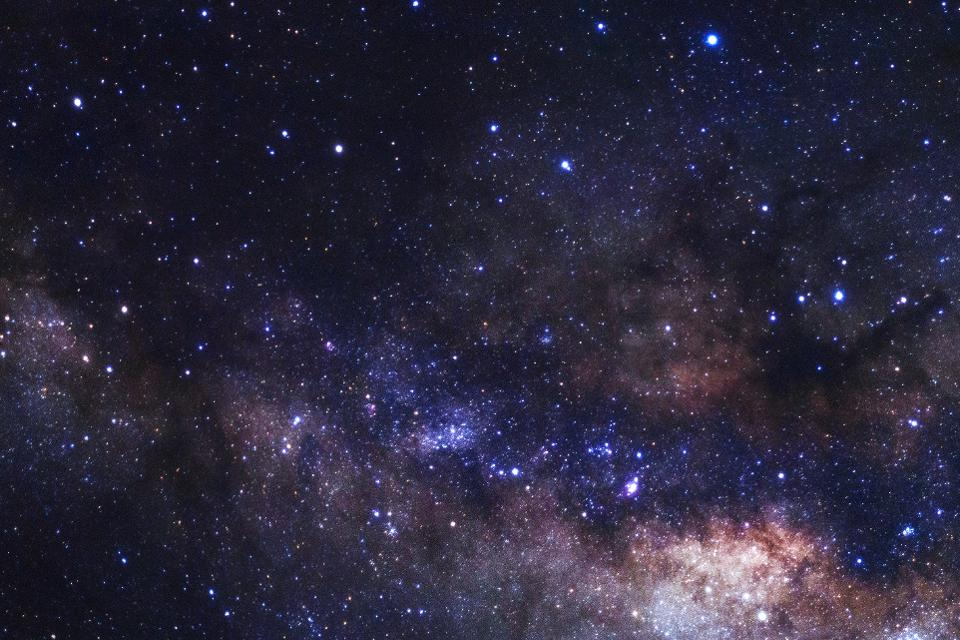
\includegraphics[width=\linewidth]{figures/space2.png}
 \captionof{figure}{Caption goes here}
\end{Figure}
\lipsum[5]

Sample figure in half of text:
\begin{wrapfigure}{l}{0.5\linewidth}
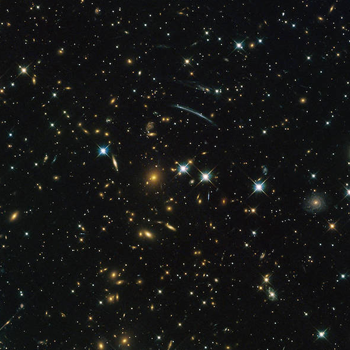
\includegraphics[width=\linewidth]{figures/space.png}
\caption{Sample picture}
\end{wrapfigure}
\lipsum[5]

%Discussion
\section{Discussion}
\lipsum[6]

%References
\section{References}
\lipsum[7]

\end{multicols}

%Author contributions
\section{Author Contributions}
\lipsum[8]

\end{document}